\documentclass[12pt,a4paper]{article}

% ================= PAQUETES =================
\usepackage[utf8]{inputenc}
\usepackage[T1]{fontenc}
\usepackage{newtxtext,newtxmath}
\usepackage[top=2.5cm, bottom=2.5cm, left=3.5cm, right=2.5cm]{geometry}
\usepackage{setspace}
\doublespacing
\usepackage{graphicx}
\usepackage{indentfirst}
\usepackage[hidelinks]{hyperref}
\usepackage{titlesec}
\usepackage{caption}
\usepackage{booktabs}
\usepackage{multirow}
\usepackage{array}
\usepackage{enumitem}
\usepackage{amsmath}
\usepackage{longtable}
\usepackage{float}
\usepackage{tabularx}

% ================= COLORES PARA TABLAS =================
\usepackage[table]{xcolor}

% ================= ALGORITMOS Y PSEUDOCÓDIGO =================
\usepackage[ruled,vlined,onelanguage]{algorithm2e}
\SetKwComment{Comment}{// }{}
\SetKwInput{KwInput}{Entrada}
\SetKwInput{KwOutput}{Salida}
\SetKwFor{ForEach}{para cada}{hacer}{fin para}
\SetKwIF{Si}{SinoSi}{Sino}{si}{entonces}{sino si}{sino}{fin si}
\SetKwFor{Para}{para}{hacer}{fin para}
\SetKwFor{While}{mientras}{hacer}{fin mientras}
\SetKwProg{Fn}{Función}{:}{fin}

% ================= SUBFIGURAS =================
\usepackage{subcaption}

% ================= FORMATO DE TÍTULOS =================
\titleformat{\section}{\normalfont\Large\bfseries\centering}{\thesection.}{1em}{\MakeUppercase}
\titleformat{\subsection}{\normalfont\large\bfseries}{\thesubsection.}{1em}{\MakeUppercase}
\titleformat{\subsubsection}{\normalfont\normalsize\bfseries}{\thesubsubsection.}{1em}{}

% ================= FORMATO DE TABLAS Y FIGURAS =================
\captionsetup[table]{labelsep=newline, textfont=it, font=normalsize, justification=raggedright, singlelinecheck=off}
\captionsetup[figure]{labelsep=newline, textfont=it, font=normalsize, justification=raggedright, singlelinecheck=off}

% ================= PÁRRAFOS =================
\setlength{\parindent}{1.25cm}
\setlength{\parskip}{10pt}

\usepackage[spanish,es-tabla]{babel}

\begin{document}
\thispagestyle{empty}
\begin{center}
    {\fontsize{18}{21}\selectfont \textbf{UNIVERSIDAD NACIONAL DEL ALTIPLANO} \par}
    \vspace{0.3cm}
    {\fontsize{14}{17}\selectfont \textbf{Árboles de Dependencia, Información Mutua y Redes Bayesianas} \par}
    \vspace{0.3cm}
    {\fontsize{14}{17}\selectfont \textbf{Predicción de Abandono Universitario} \par}
    \vspace{0.5cm}
    {\fontsize{12}{15}\selectfont JAHUIRA PONCE CHRISTIAN SEBASTIÁN \par}
    \vspace{0.3cm}
    {\fontsize{12}{15}\selectfont PUNO -- PERÚ -- 2026 \par}
\end{center}
\newpage
\section{Redes Bayesianas -- Algoritmo de Chow-Liu}

El árbol de dependencias construido mediante Información Mutua y el algoritmo de Kruskal es, de hecho, el resultado del \textbf{algoritmo de Chow-Liu} para el aprendizaje de la estructura de una red Bayesiana. Chow-Liu (1968) demostró que la estructura de árbol que maximiza la verosimilitud de los datos es exactamente el Árbol de Expansión de Peso Máximo calculado sobre la matriz de Información Mutua. En otras palabras, el MST obtenido en las secciones anteriores es la \textbf{estructura óptima de red Bayesiana tipo árbol} para este dataset.

\subsection{Construcción del DAG}

Para convertir el MST (grafo no dirigido) en una red Bayesiana (grafo dirigido acíclico, DAG), se selecciona el nodo \texttt{Target} como raíz y se orientan todas las aristas alejándose de él mediante un recorrido en anchura (BFS). El resultado es el siguiente DAG:

\begin{figure}[H]
    \centering
    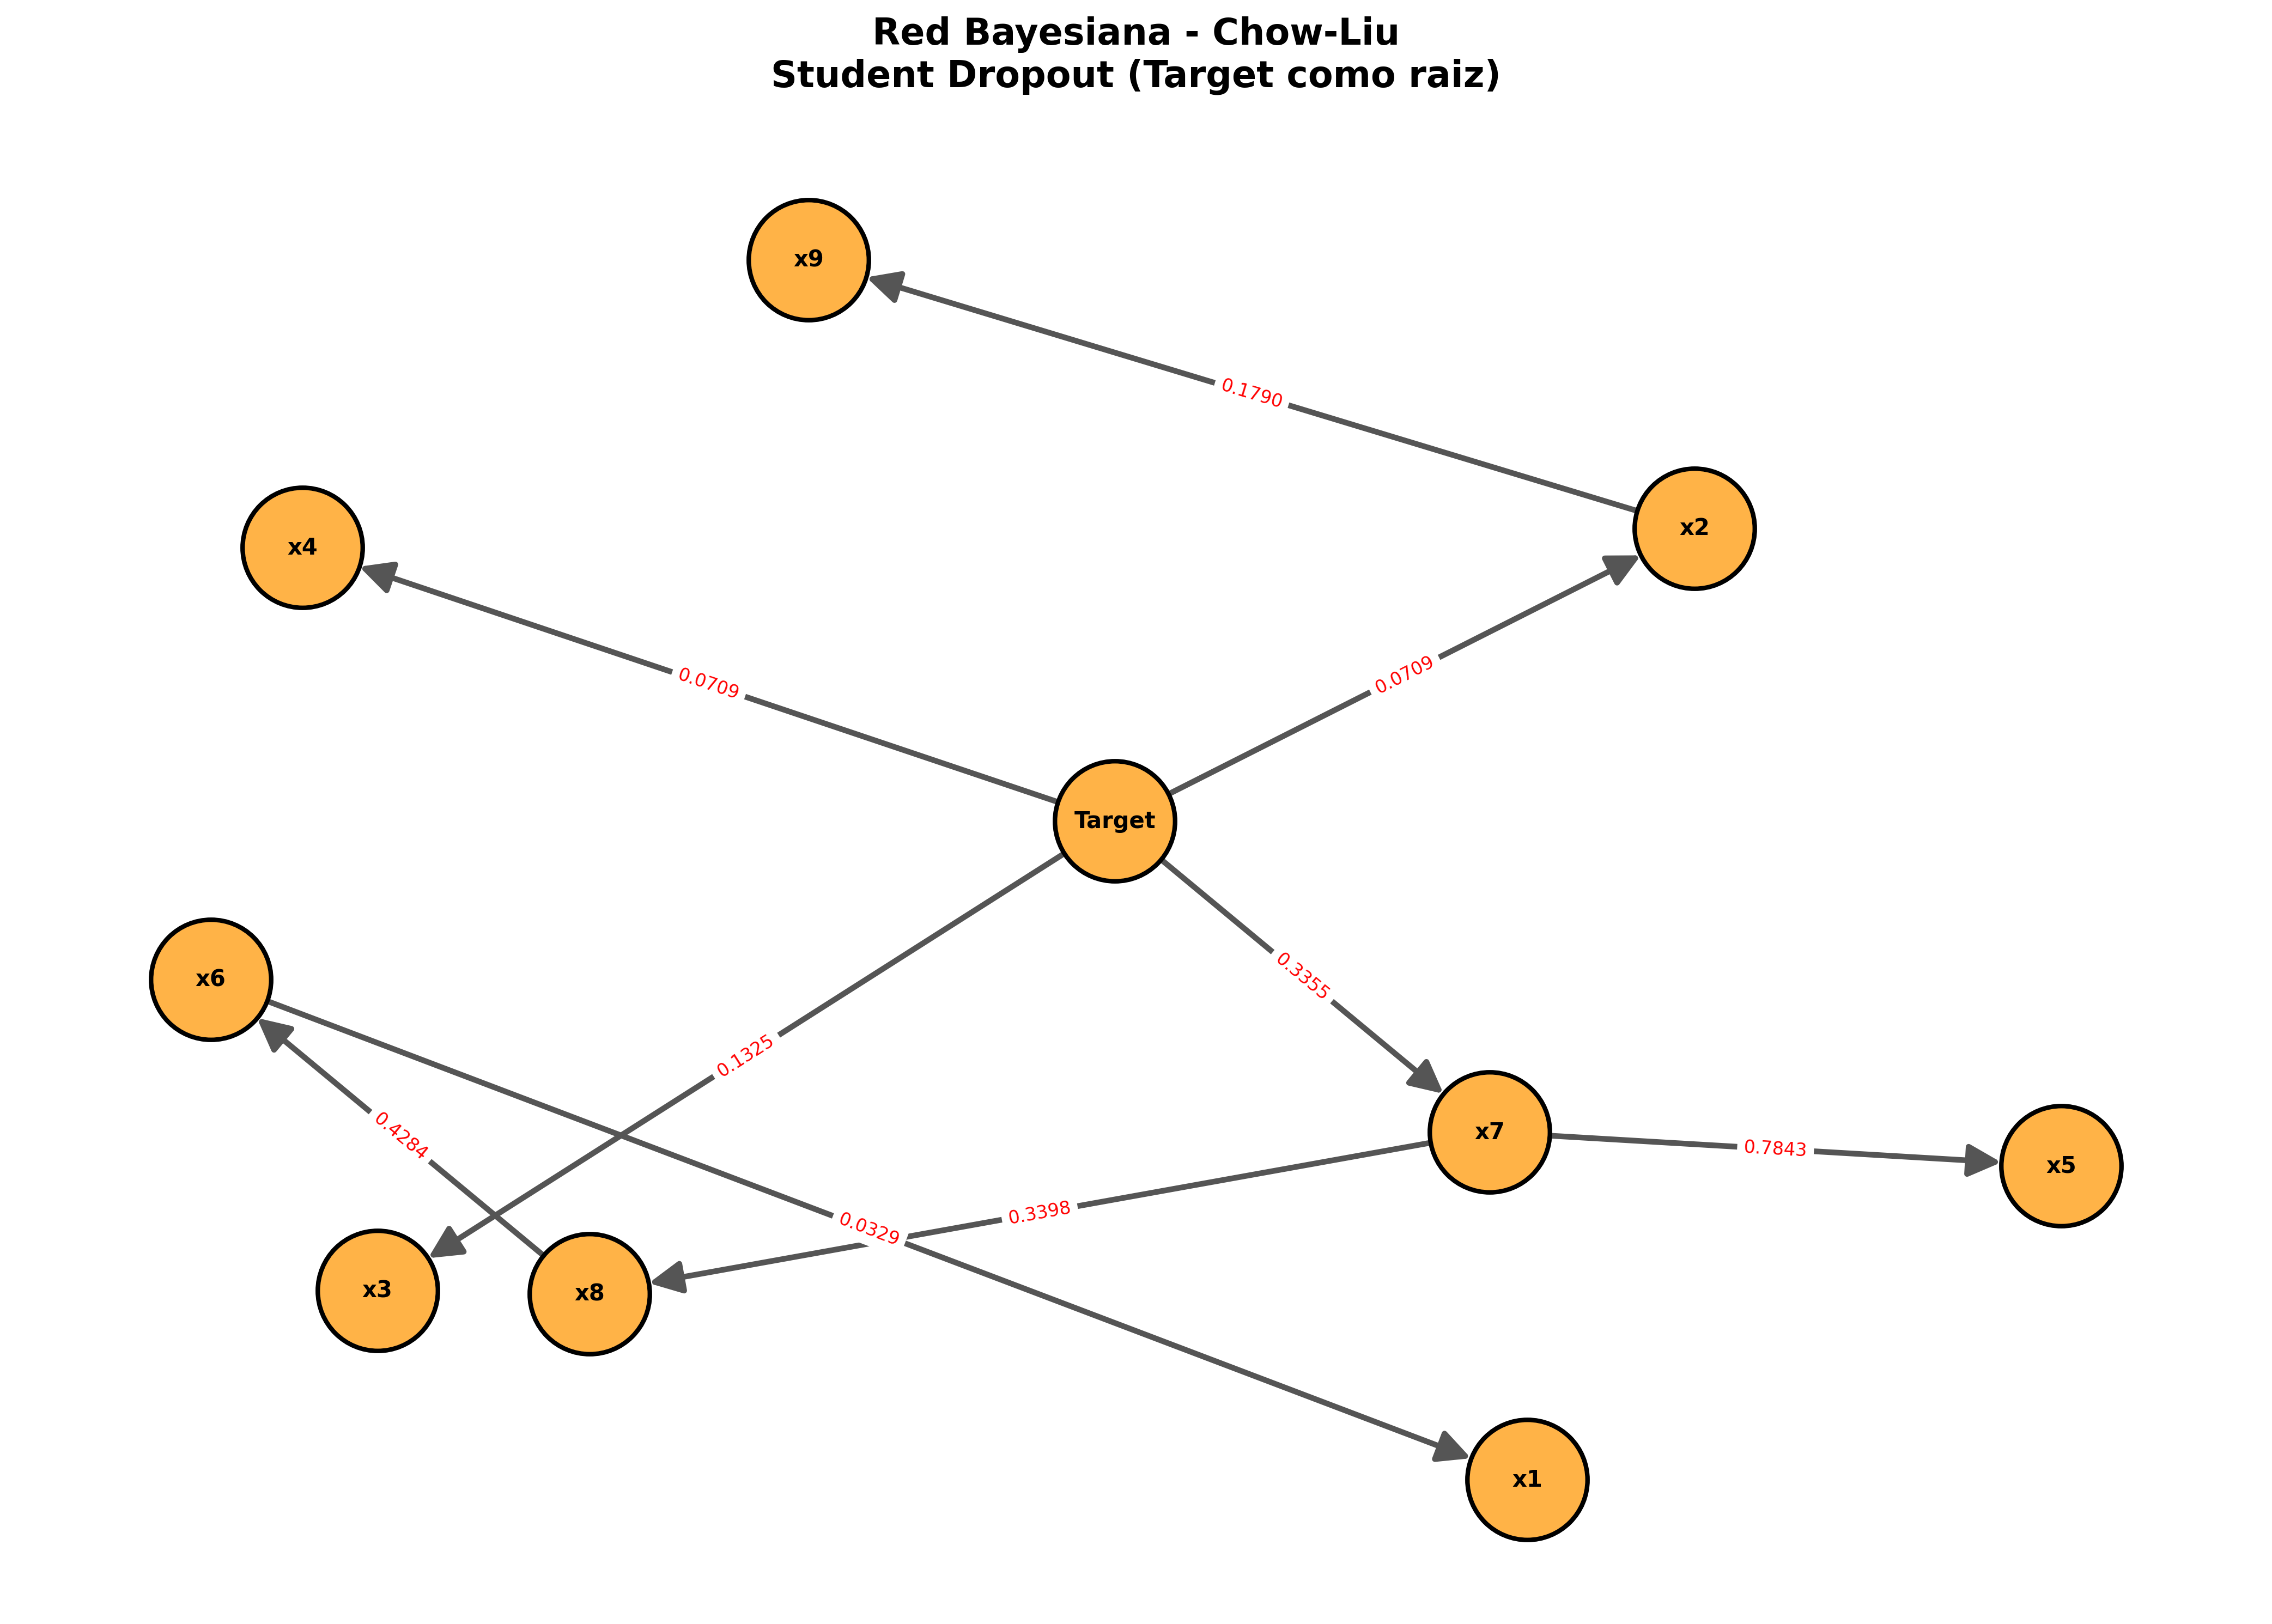
\includegraphics[width=0.85\textwidth]{red_bayesiana.png}
    \caption{Red Bayesiana aprendida mediante Chow-Liu. Target como nodo raíz. Las aristas están dirigidas desde Target hacia las hojas.}
    \label{fig:bayes}
\end{figure}

La estructura dirigida obtenida (usando el dataset original con 4,424 registros) es:

\begin{table}[H]
    \centering
    \begin{tabular}{lll}
        \toprule
        \textbf{Arco} & \textbf{Variable hija} & \textbf{Peso MI} \\
        \midrule
        Target $\rightarrow$ $x_7$ & Aprobados 2do semestre & 0.3355 \\
        Target $\rightarrow$ $x_3$ & Pagos al día & 0.1325 \\
        Target $\rightarrow$ $x_4$ & Becado & 0.0709 \\
        Target $\rightarrow$ $x_2$ & Edad & 0.0709 \\
        $x_7$ $\rightarrow$ $x_5$ & Aprobados 1er semestre & 0.7843 \\
        $x_7$ $\rightarrow$ $x_8$ & Nota 2do semestre & 0.3398 \\
        $x_8$ $\rightarrow$ $x_6$ & Nota 1er semestre & 0.4284 \\
        $x_6$ $\rightarrow$ $x_1$ & Nota de admisión & 0.0329 \\
        $x_2$ $\rightarrow$ $x_9$ & Estado civil & 0.1790 \\
        \bottomrule
    \end{tabular}
    \caption{Estructura del DAG aprendido (Chow-Liu sobre dataset original).}
\end{table}

\subsection{Tablas de Probabilidad Condicional (CPTs)}

Para los nodos conectados directamente al Target, se calculan las distribuciones de probabilidad condicional. Estas CPTs permiten realizar inferencia en la red.

\subsubsection{CPT: $P(x_7 \mid Target)$}

\begin{table}[H]
    \centering
    \begin{tabular}{c|ccc}
        \toprule
        \textbf{Target} & $P(x_7=0)$ & $P(x_7=1)$ & $P(x_7=2)$ \\
        \midrule
        Dropout (0) & 0.8220 & 0.1288 & 0.0493 \\
        Enrolled (1) & 0.5756 & 0.3212 & 0.1033 \\
        Graduate (2) & 0.1159 & 0.5672 & 0.3169 \\
        \bottomrule
    \end{tabular}
    \caption{Probabilidad condicional de aprobados en 2do semestre dado el Target.}
\end{table}

Interpretación: Si un estudiante abandona (Dropout), hay un $82.2\%$ de probabilidad de que tenga bajo rendimiento ($x_7 = 0$) en el segundo semestre. Si se gradúa, solo un $11.6\%$ tiene bajo rendimiento.

\subsubsection{CPT: $P(x_3 \mid Target)$}

\begin{table}[H]
    \centering
    \begin{tabular}{c|cc}
        \toprule
        \textbf{Target} & $P(x_3=0)$ & $P(x_3=1)$ \\
        \midrule
        Dropout (0) & 0.3216 & 0.6784 \\
        Enrolled (1) & 0.0529 & 0.9471 \\
        Graduate (2) & 0.0131 & 0.9869 \\
        \bottomrule
    \end{tabular}
    \caption{Probabilidad condicional de pagos al día dado el Target.}
\end{table}

Interpretación: Los estudiantes que abandonan tienen un $32.2\%$ de probabilidad de no tener los pagos al día, frente a solo $1.3\%$ de los graduados.

\subsection{Ejemplo de Inferencia}

Utilizando las CPTs y la estructura del DAG, es posible realizar inferencia probabilística. A continuación se presenta un ejemplo de inferencia directa desde los datos:

\textbf{Pregunta:} ¿Cuál es la probabilidad de abandono para un estudiante con baja nota de admisión ($x_1 = 0$) y que no tiene los pagos al día ($x_3 = 0$)?

\begin{align*}
    P(Target = Dropout \mid x_1 = 0, x_3 = 0) &= 0.9207 \quad (92.1\%) \\
    P(Target = Enrolled \mid x_1 = 0, x_3 = 0) &= 0.0573 \quad (5.7\%) \\
    P(Target = Graduate \mid x_1 = 0, x_3 = 0) &= 0.0220 \quad (2.2\%)
\end{align*}

Este resultado muestra que la combinación de baja nota de admisión y falta de pago es un predictor extremadamente fuerte de abandono universitario: más del $92\%$ de los estudiantes con este perfil terminan abandonando.

\subsection{Conclusiones de la Red Bayesiana}

\begin{itemize}
    \item El algoritmo de Chow-Liu proporciona una estructura de red Bayesiana que es \textbf{exactamente el MST} calculado en las secciones anteriores, validando la coherencia entre ambos enfoques.
    \item La orientación desde Target como raíz revela una \textbf{jerarquía natural}: el Target influye directamente sobre variables financieras ($x_3$, $x_4$) y de rendimiento ($x_7$), que a su vez influyen sobre otras variables académicas en cascada.
    \item Las CPTs permiten \textbf{cuantificar el riesgo} de abandono para perfiles específicos de estudiantes, lo cual tiene aplicaciones prácticas en sistemas de alerta temprana.
    \item La red Bayesiana obtenida es un modelo \textbf{explicable e interpretable}, donde cada arco tiene un significado causal plausible en el contexto educativo.
\end{itemize}

% =============================================
% ANEXOS
% =============================================
\newpage
\section{Anexos: Código Fuente}

El código fuente completo del proyecto (Python, LaTeX, datos y resultados) está disponible en el repositorio de GitHub:

\begin{center}
    \url{https://github.com/HidenXye/Lenguajes-Split}
\end{center}

El archivo \texttt{resolucion\_dropout.py} implementa: carga y discretización de variables, cálculo de entropía paso a paso, matriz de Información Mutua, construcción del MST mediante los algoritmos de Kruskal y Prim, análisis de sensibilidad rVP con distancias de camino, y aprendizaje de la red Bayesiana mediante el algoritmo de Chow-Liu.


\end{document}
